\section{NE555}

Maintenant que nous avons transformé les pics en signaux rectangulaires, il nous reste à utiliser ces dernières afin de générer une impulsion \textit{unique}. Pour cela, nous allons utiliser un composant particulier: le \texttt{NE555}. Bien que commercialisé en 1971, ce composant est toujours utilisé de nos jours en raison de la multitude de modes de fonctionnement qu'il offre, ainsi que sa facilité d'utilisation. Aujourd'hui, nous allons utiliser ce dernier en mode dit \textbf{monostable} afin de générer une impulsion de durée déterminée. \\

Le montage que nous allons réaliser est représenté à la Figure \ref{fig:mono555}. Initialement, la tension de sortie a une valeur logique basse. Lorsqu'une impulsion descendante se produit à l'entrée \texttt{TRIG} (e.g. la fin d'un signal rectangulaire), la borne de décharge \texttt{DISCH} est désactivée, permettant ainsi à la capacité $C2$ de se charger à travers la résistance $R5$. Lors de cette charge, la tension de sortie du noeud \texttt{OUT3} a une valeur logique haute. Après un temps de charge $t_c$, la tension aux bornes de $C2$ dépasse la valeur seuil (i.e. $2/3V_{CC}$) ce qui a pour effet de repasser la valeur de la tension de sortie à 0 et de réactiver la borne de décharge \texttt{DISCH}. La valeur du temps de charge $t_c$ est donné par:

\begin{equation}
    t_c = 1.1 \cdot R_5 \cdot C_2
\end{equation}

De manière plus pratique, le \texttt{NE555} que nous allons utiliser est le \texttt{NE555N} fabriqué par \textsc{STMicroelectronics}. Un petit coup d'oeil sur la datasheet peut être interressant pour connaitre la configuration du composant. 

\begin{figure}[h!]
    \centering
    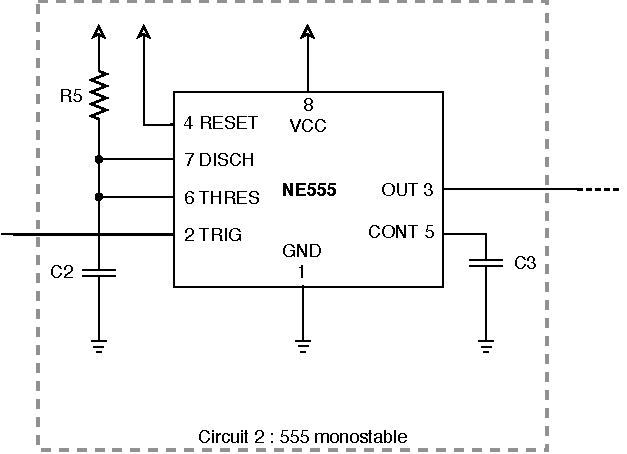
\includegraphics[width=0.7\textwidth]{HO2_555.pdf}
    \caption{Montage monostable du NE555}
    \label{fig:mono555}
\end{figure}